\newpage
\section{Bode Plots}
Bode plots are used to evaluate the behaviour of closed-loop systems.
\begin{itemize}
    \item \textbf{Gain plot} 
    \[
        20\log_{10}\lvert G(j\omega) \rvert \ \text{\textcolor{gray}{[in dB]}}\quad \text{v.s.} \quad \omega \ \textcolor{gray}{(\text{in } \log_{10} \ \text{scale})}
    \]
    
    \item \textbf{Phase plot} 
    \[
        \angle G(j\omega) \ \text{\textcolor{gray}{[in deg]}} \quad \text{v.s.} \quad \omega \ \textcolor{gray}{(\text{in } \log_{10} \ \text{scale})}  
    \]
\end{itemize}
The Bode plots of a complex system can be obtained by the addition of Bode plots for simple systems.
\begin{itemize}
    \item For gain plot:
    \[
        20\log_{10}\lvert G(j\omega)\rvert  = 20\log_{10}\lvert G_{1}(j\omega)\rvert+20\log_{10}\lvert G_{2}(j\omega)\rvert
    \]
    
    \item For phase plot:
    \[
        \angle G(j\omega) = \angle G_{1}(j\omega)+\angle G_{2}(j\omega)
    \]
\end{itemize}

\subsection{Bode Plots for Constant Gain, $G(s) = K$}
\begin{itemize}
    \item \textbf{Gain plot}: $20\log_{10}\lvert G(j\omega) \rvert \ = 20\log_{10}K$ 
    \item \textbf{Phase plot}: $\angle G(j\omega) = 0^{\circ}$
\end{itemize}

\begin{figure}[H] 
    \centering 
    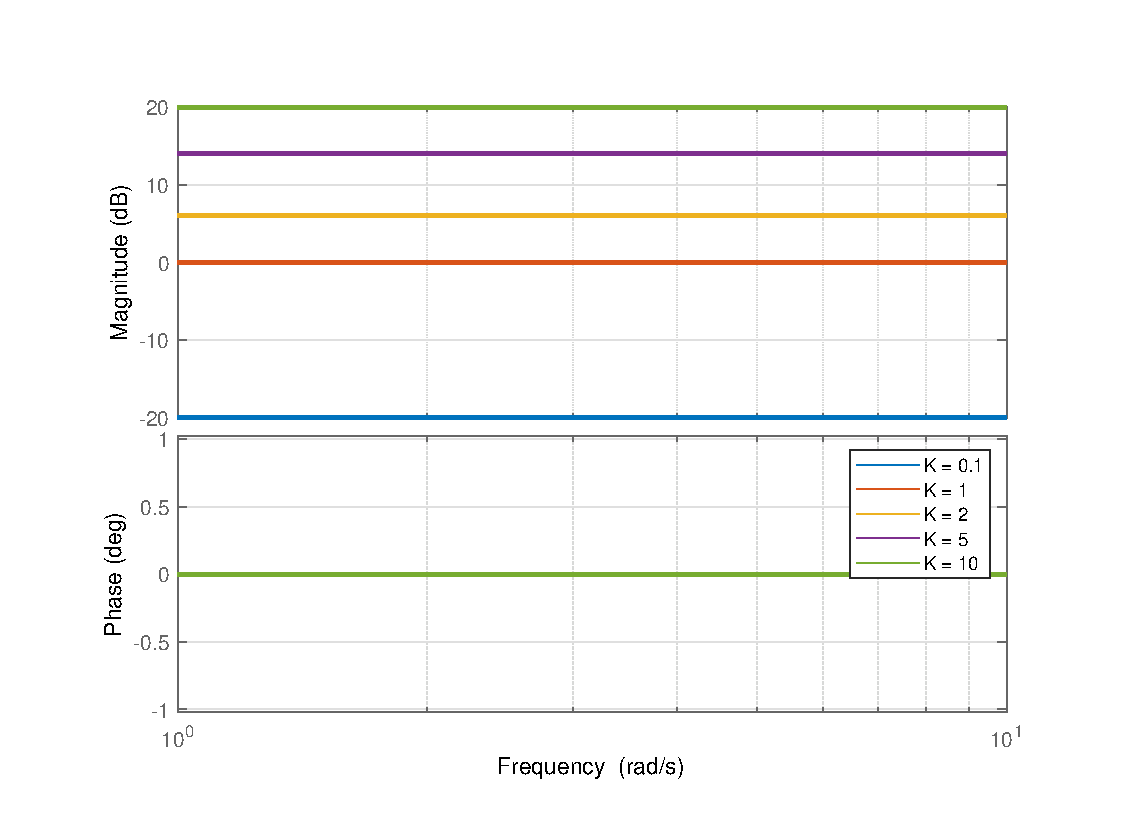
\includegraphics[width=.7\textwidth]{images/bode5.eps}
    \caption{Bode plot of $G(s) = K$. Magnitude plot is a constant.}
\end{figure}

\subsection{Bode Plots for Differentiator, $G(s) = s^{n}$}
\begin{itemize}
    \item \textbf{Gain plot}: 
    \[
        20\log_{10}\lvert G(j\omega) \rvert  = 20\log_{10}\lvert (j\omega)^{n} \rvert = n\cdot 20\log_{10}\lvert (j\omega) \rvert=\boxed{n\cdot20\log_{10}\omega}
    \]
    
    \item \textbf{Phase plot}: $\angle G(j\omega) = \angle (j\omega)^{n} = \boxed{n\cdot 90^{\circ}}$
    
    \item Gain difference $\Delta$ over the interval $[\omega_{1}, \omega_{2}] $: 
    \[
        \Delta = n\cdot20(\log_{10}\omega_{1}-\log_{10}\omega_{2})=\boxed{n\cdot20 \log_{10}\frac{\omega_{1}}{\omega_{2}}}
    \]
    This gives the slope$=n\cdot 20$ \textcolor{gray}{[dB/decade]}
\end{itemize}

\begin{figure}[H] 
    \centering 
    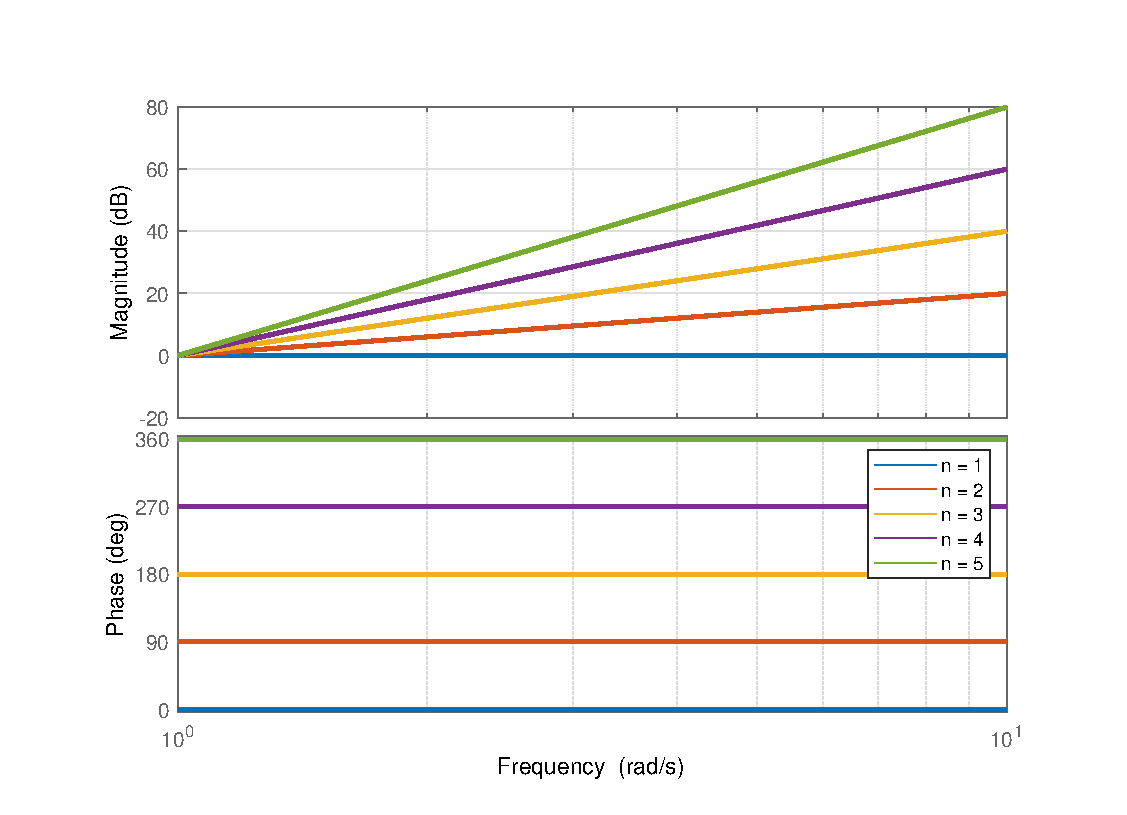
\includegraphics[width=.7\textwidth]{images/bode6.eps}
    \caption{Bode plot of $G(s) = s^{n}$.}
\end{figure}

\subsection{Bode Plots for Integrator, $G(s) = (\frac{1}{s})^{n}$}
\begin{itemize}
    \item \textbf{Gain plot}:
    \[
        20\log_{10}\lvert G(j\omega) \rvert
        = 20 \log_{10} \lvert (\frac{1}{j\omega})^{n} \rvert 
        = -n \cdot 20 \log_{10} \lvert (j\omega) \rvert
        = \boxed{-n\cdot20\log_{10}\omega}
    \]
    
    \item \textbf{Phase plot}: $\angle G(j\omega) = \angle (\frac{1}{j\omega})^{n} = \boxed{-n\cdot 90^{\circ}}$
    
    \item Gain difference $\Delta$ over the interval $[\omega_{1}, \omega_{2}] $: 
    \[ 
        \Delta = -n\cdot20(\log_{10}\omega_{1}-\log_{10}\omega_{2})=\boxed{-n\cdot20 \log_{10}\frac{\omega_{1}}{\omega_{2}}}
    \]
    This gives the slope$=-n\cdot 20$ \textcolor{gray}{[dB/decade]}
\end{itemize}

\begin{figure}[H] 
    \centering 
    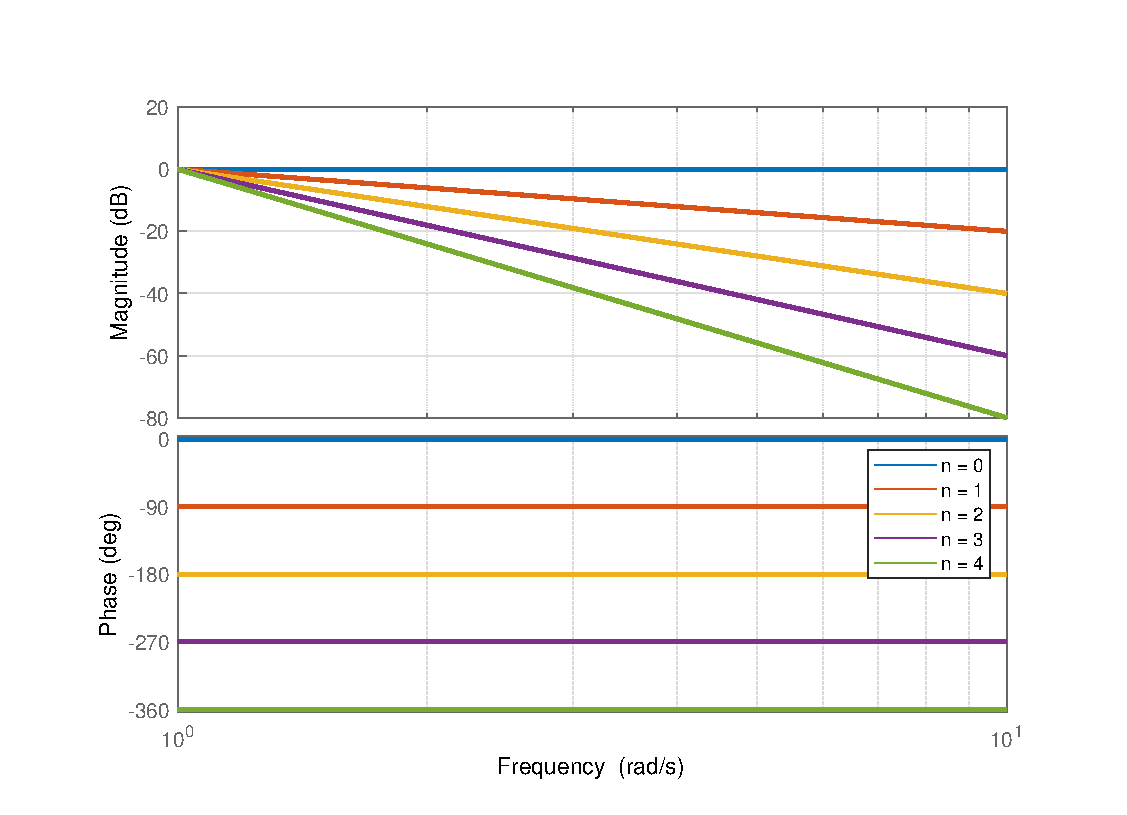
\includegraphics[width=.7\textwidth]{images/bode4.eps}
    \caption{Bode plot of  $G(s) = (\frac{1}{s})^{n}$.}
\end{figure}

\subsection{Bode Plots for 1\textsuperscript{st} Order System, $G(s) = \frac{K}{Ts+1}$}
\begin{itemize}
    \item \textbf{Gain plot}: 
    \begin{align*}
    \begin{split}
    20 \log_{10} \lvert G(j\omega) \rvert  
    & = 20\log_{10} \lvert \frac{K}{Ts+1} \rvert 
    = 20\log K-20\log\sqrt{T^{2}\omega^{2}+1} \\
    & \approx 
    \begin{cases} 
        20 \log K                   & T\omega<<1\\
        20 \log K - 20\log T\omega  & T\omega>>0
    \end{cases} 
    \end{split} 
    \end{align*}
    
    \item \textbf{Phase plot}: 
    \[
        \angle G(j\omega) \= \angle \frac{1}{Tj\omega+1}=\frac{-T\omega j +1}{T^{2}\omega^{2}+1}=\tan^{-1}(-T\omega)\approx 
        \begin{cases}
            0^{\circ}   & T\omega<<1\\
            -45^{\circ} & \omega=\omega_{c}=\frac{1}{T}\\
            -90^{\circ} & T\omega>>0
        \end{cases}
    \]
    
    \item Gain difference $\Delta$ over the interval $[\omega_{1}, \omega_{2}] $: \[ \Delta = -20(\log_{10}\omega_{1}-\log_{10}\omega_{2})=\boxed{-20 \log_{10}\frac{\omega_{1}}{\omega_{2}}}\]
    This gives the slope$=- 20$ \textcolor{gray}{[dB/decade]}
    
    \item Corner frequency: $20\log T\omega_{c}=0 \to \omega_{c} = \frac{1}{T}$

    \begin{figure}[H] 
        \centering 
        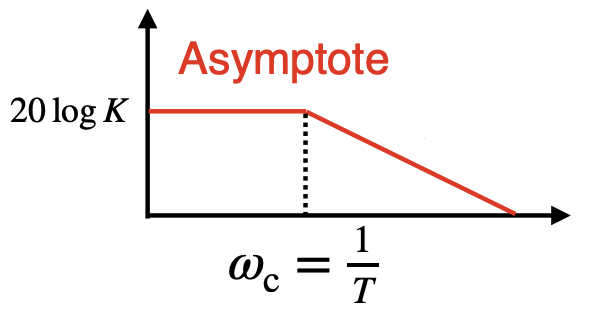
\includegraphics[width=.3\textwidth]{images/corner_1.png}
        \caption{Corner frequency, $\omega_{c}$}
    \end{figure}
    
    \begin{figure}[H]
        \centering 
        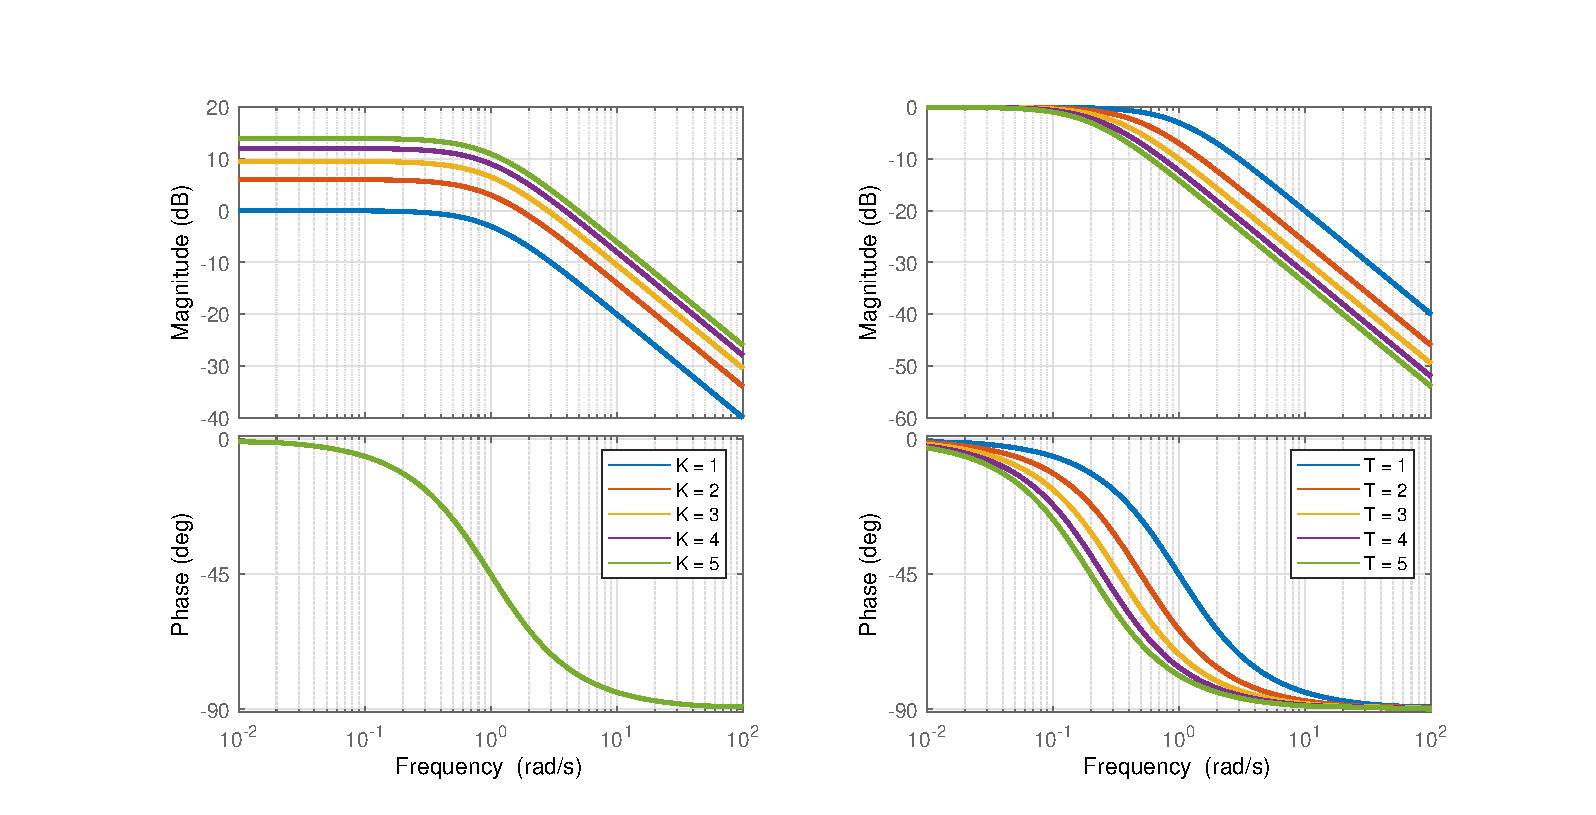
\includegraphics[width=1\textwidth]{images/bode3.eps}
        \caption{Bode plot for $G(s) = \frac{K}{Ts+1}$. \textbf{Left: $T=1$, $K\in [1,5]$. Right: $K=1$, $T\in [1,5]$.}}
    \end{figure}
\end{itemize}

\subsection{Bode Plots for 1\textsuperscript{st} Order Factor, $G(s) = (Ts+1)^{n}$}
\begin{itemize}
    \item \textbf{Gain plot}:
    \[
        20\log_{10}\lvert G(j\omega) \rvert
        = n\cdot 20\log_{10} \lvert Tj\omega+1 \rvert 
        = n\cdot20\log\sqrt{T^{2}\omega^{2}+1}\approx 
        \begin{cases}
            0                       & T \omega << 1\\
            n\cdot 20\log T\omega   & T \omega >> 0
        \end{cases}
    \]
    
    \item \textbf{Phase plot}:
    \[
        \angle G(j\omega) 
        = \angle (Tj\omega+1)^{n} 
        = n\cdot \tan^{-1}(T\omega) \approx 
        \begin{cases}
            0^{\circ}           & T\omega<<1\\
            n\cdot 45^{\circ}   & \omega=\omega_{c}=\frac{1}{T}\\
            n\cdot 90^{\circ}   & T\omega>>0\\
        \end{cases}
    \]
    
    \item Corner frequency $\omega_{c} = \frac{1}{T}$, \ slope = $n\cdot 20$ \textcolor{gray}{[dB/decade]}
\end{itemize}

\begin{figure}
    \centering
    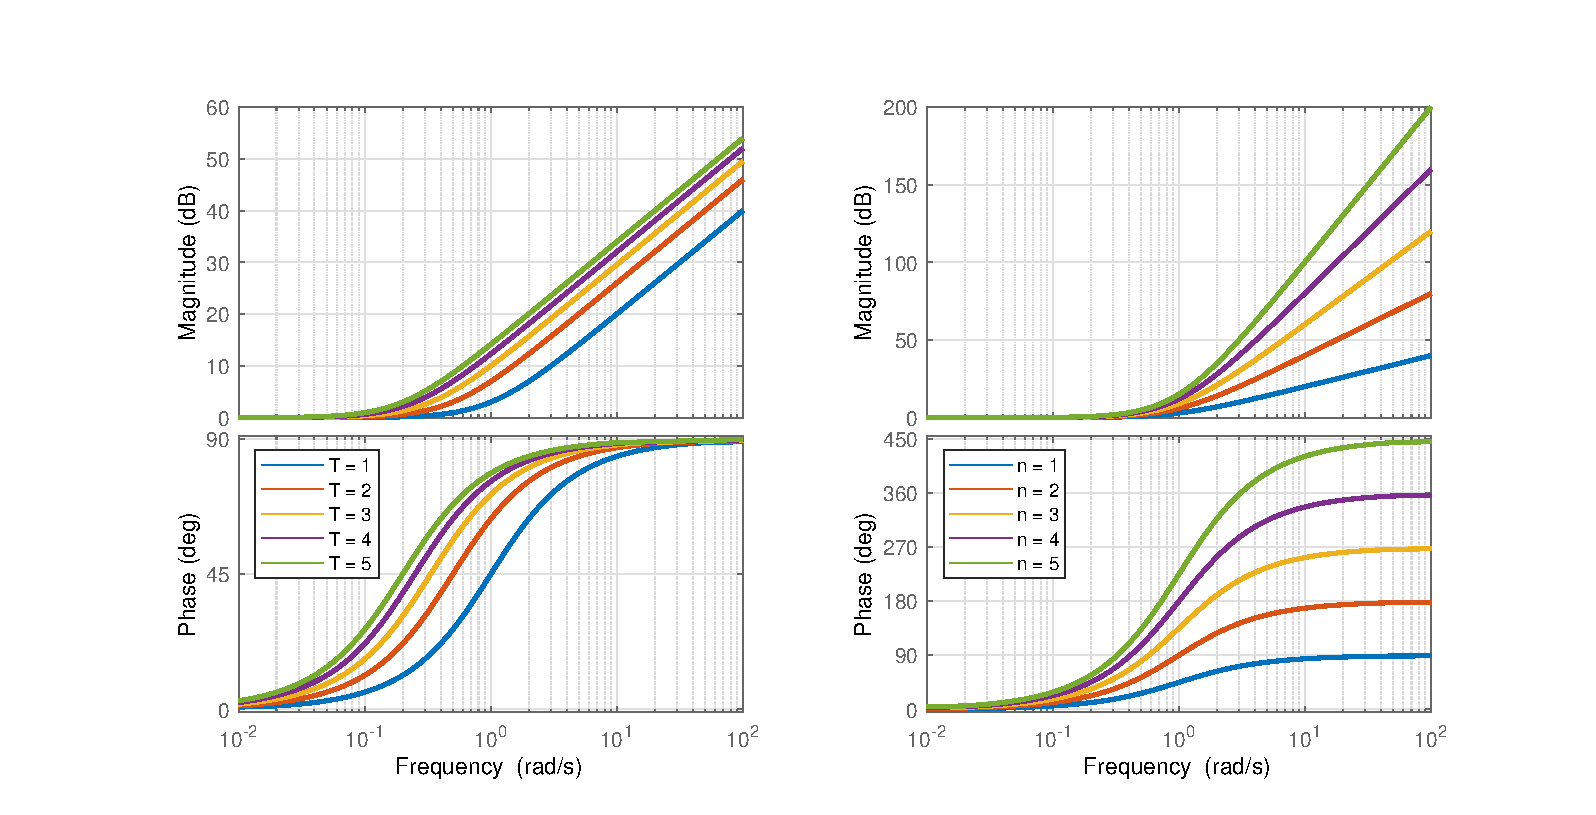
\includegraphics[width=\textwidth]{images/bode2.eps}
    \caption{Bode plot for $G(s) = (Ts+1)^{n}$. \textbf{Left: $n=1$, $T\in [1,5]$. Right: $T=1$, $n\in [1,5]$.}}
\end{figure}

\subsection{Bode Plots for 2\textsuperscript{nd} Order System, $G(s) = \frac{K\omega_{n}^{2}}{s^{2}+2\zeta\omega_{n}s+\omega_{n}^{2}}$}
Write the transfer function as a product of basic factors:
\[
    G(s) = \frac{K\omega_{n}^{2}}{s^{2}+2\zeta\omega_{n}s+\omega_{n}^{2}}=\frac{K}{-r^{2}+2\zeta jr +1}=\frac{K}{(1-r^{2})+2j\zeta r}
\]
where $r$ is known as the normalized frequency: $r = \frac{\omega}{\omega_{c}}$.

\begin{itemize}
    \item \textbf{Bode plot}:
    \[
        20\log_{10}\lvert G(j\omega) \rvert  =  20\log_{10} \bigg\lvert \frac{K}{(1-r^{2})+2j\zeta r} \bigg\rvert \approx 
        \begin{cases}
            20\log K            & r<<1 \\
            20\log K - 40\log r & r>>0
        \end{cases}
    \]

    \item \textbf{Phase plot}:
    \[
        \angle G(j\omega) = \angle \frac{K}{(1-r^{2})+2j\zeta r} =  \tan^{-1}(\frac{-2r\zeta}{1-r^{2}}) \approx 
        \begin{cases}
            0^{\circ}       & r<<1\\
            -90^{\circ}     & r = r_{c} = 1\\
            -180^{\circ}    & r>>0\\
        \end{cases}
    \]
    
    \item Resonant frequency $\omega_{r}$ at which the magnitude becomes max:
    \[
        \frac{d\lvert G(j\omega) \rvert}{dr}=0 \to r^{2} = q-2\zeta^{2}
    \]
    \[
        \omega_{r} = \omega_{n}\sqrt{1-2\zeta^{2}}
    \]
    Resonant peak magnitude at $\lvert G(j\omega_{r}) \rvert =\frac{1}{2\zeta\sqrt{1-\zeta^{2}}} $
\end{itemize}
%plots starts here!
\vspace{-.6cm}
\begin{figure}[H]
    \centering
    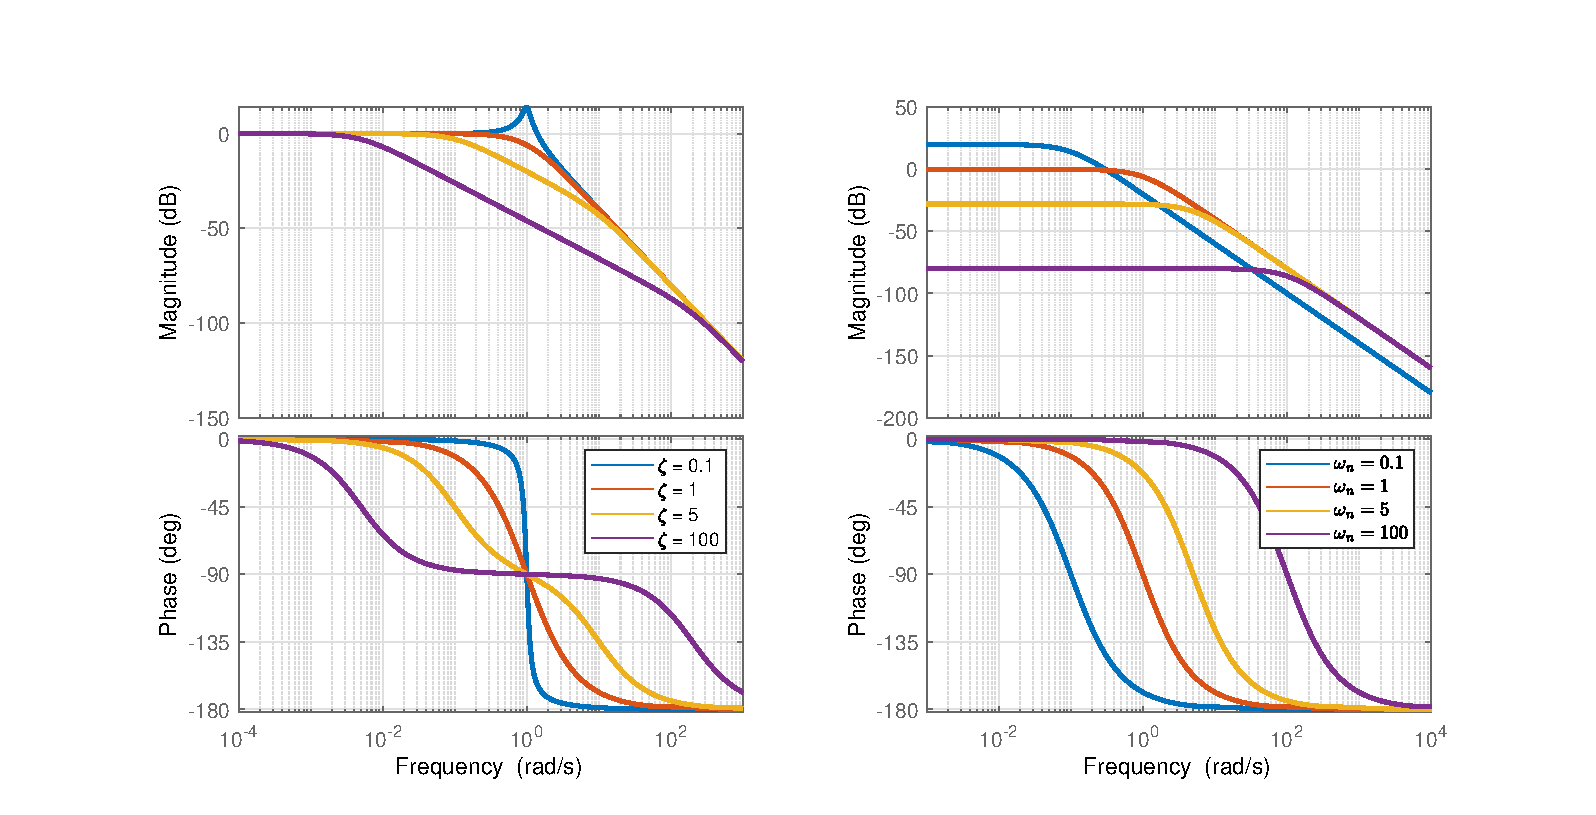
\includegraphics[width=\textwidth]{images/bode1.eps}
    \caption{Bode plot for $G(s) = \frac{K\omega_{n}^{2}}{s^{2}+2\zeta\omega_{n}s+\omega_{n}^{2}}$. \textbf{Left:} $\omega_{n}=1$, $\zeta$ varies. \textbf{Right:} $\zeta=1$, $\omega_{n}$ varies.}
\end{figure}

\subsection{Drawing Approximate Bode Plots}
\begin{enumerate}
\item Write the transfer function as a product of basic factors;
%---------------EXAMPLE START---------------%
    \begin{tcolorbox}[breakable, title=Example]
        \[G(s) = \frac{s+5}{(s+2)(s+4)}=\frac{5(0.2s+1)}{2(0.5s+1).4(0.25s+1)} = \frac{0.625. (0.2s+1)}{(0.5s+1)(0.25s+1)}\]
    \end{tcolorbox}
%----------------EXAMPLE END----------------%

    \item Identify the corner frequency for each factor;
%---------------EXAMPLE START---------------%
    \begin{tcolorbox}[breakable, title=Example cont'd]
        \[\omega_{c} = \frac{1}{0.5} , \frac{1}{0.25} , \frac{1}{0.2} = 2,4,5\]
    \end{tcolorbox}
%----------------EXAMPLE END----------------%

    \item Draw the \textbf{asymptotes between the corner frequencies} and \textbf{add the individual plots}.
        \begin{figure}[H] 
            \centering
            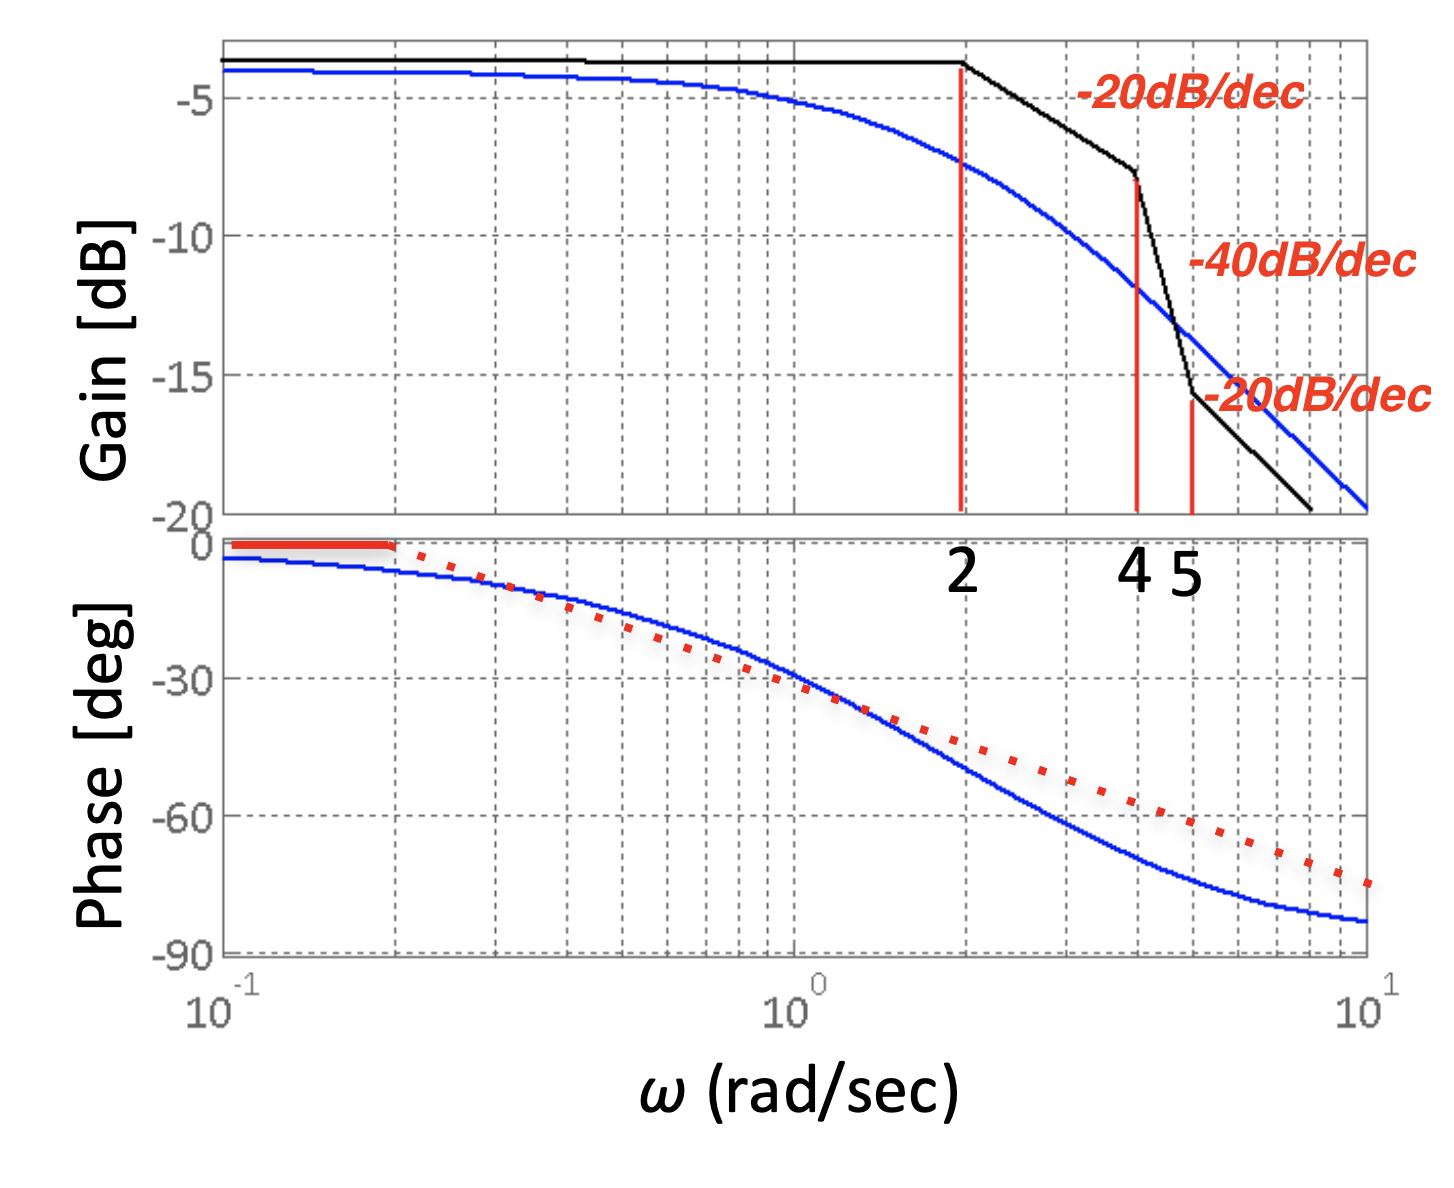
\includegraphics[width=.5\textwidth]{images/bode_plot.png}
        \end{figure}
\end{enumerate}